% =========================================================================
% CHAPTER 7
% =========================================================================

\chapter{Evaluierung}
\label{K7}
Zur Evaluierung werden zwei konkrete JobScripts herangezogen: ein Script, das einen Bereich der natürlichen Zahlen nach Primzahlen durchsucht (siehe Experiment \ref{M1}), und ein weiteres, das einen 3D Processing Algorithmus auf mehrere Input-Dateien anwendet (siehe Experiment \ref{M2}, \ref{M3}).
Als Hardware standen fünf Rechner mit gleicher Ausstattung, jeweils 4 Cores und 16GB RAM, zur Verfügung. Pro Rechner wurden maximal vier Worker verwendet um Swapping zu vermeiden, denn die JobScripts verwenden nur einen primitiven Scheduler.
Gemessen wurden neben der Gesamtlaufzeit auch die Laufzeiten der SubJobs, jeweils immer auf dem Rechner auf dem sie erstellt wurden - bei RemoteJobs bedeutet das inklusive des Netzwerk Roundtrips.

Ziel der Messungen ist es zu zeigen, inwiefern das System beziehungsweise das JobScript skaliert. Als Betriebssystem wurde Linux verwendet, allerdings keine Realtime Variante, was ein Schwanken der Messergebnisse zur Folge hatte. Deshalb wurden alle Messungen 25 mal durchgeführt.

Für die folgenden Experimente wird jeweils ein Histogram der WorkerJob Laufzeiten und ein Boxplot der Gesamtlaufzeit für ein, zwei und vier Rechner gezeigt. Weiters wird die Gesamtlaufzeit über der Rechneranzahl auch mit logarithmischen Achsen gezeigt, da in dieser Darstellungsform eine lineare Funktion die lineare Skalierbarkeit besser sichtbar macht.





\clearpage
\section{Primzahlen Suche - Parallel Workflow}
\label{M1}

\begin{wrapfigure}{r}{0.45\textwidth}
  \vspace{-30pt}
  \begin{center}
    \includegraphics{hist-workerPrimeCpp}
    \caption{Experiment \ref{M1} WorkerJob Laufzeiten aller 25 Iterationen in 50bins.}
    \label{hist-workerPrimeCpp}
  \end{center}
\end{wrapfigure}

Dieses Experiment wurde ausgewählt, weil es einen sehr einfachen Fall zeigt, der auch gut skaliert.
Der Algorithmus durchsucht einen Bereich der natürlichen Zahlen nach Primzahlen und übergibt die Anzahl der gefundenen Primzahlen an den Client.

Der Serverteil des JobScripts teilt den zu durchsuchenden Bereich proportional auf die zur Verfügung stehenden Worker auf.
Somit ist die Anzahl der WorkerJobs immer gleich der Anzahl der Worker.
Stehen mehr Worker zur Verfügung, wird der zu durchsuchende Bereich für jeden Worker kleiner.
Histogramm \ref{hist-workerPrimeCpp} zeigt, dass mittlere WorkerJob Laufzeit annähernd linear mit der Anzahl der verfügbaren Worker sinkt.
Die Gesamtlaufzeit zeigt die erwartete lineare Skalierbarkeit, ersichtlich in Abbildung \ref{runtime-box-workerPrimeCpp} und \ref{runtime-log-workerPrimeCpp}.

Wie in Abschnitt \ref{overload} diskutiert wurde, besteht diese lineare Skalierbarkeit aber nur, sofern die WorkerJobs längere Laufzeiten haben, denn bei sehr kurzen Laufzeiten der WorkerJobs werden Return Messages in kürzeren Abständen gesendet und der Server wird überlastet.

Scheduling Probleme müssen bei parallelen Workflows nur dann nicht beachtet werden, falls gleich große Teile des Datasets gleich lange Laufzeiten aufweisen. Bei der Primzahlensuche ist dies im Detail betrachet nicht der Fall, weil großere Zahlen eine größere Laufzeit veruhrsachen.


\vspace{50mm}

\begin{figure}[H]
  \centering
  \begin{minipage}[b]{0.45\textwidth}
    \includegraphics[width=\textwidth]{runtime-box-workerPrimeCpp}
    \caption{Experiment \ref{M1}. Boxplots für Gesamtlaufzeit mit 1, 2, und 4 Worker, und je 25 Iterationen}
    \label{runtime-box-workerPrimeCpp}
  \end{minipage}
  \hfill
  \begin{minipage}[b]{0.45\textwidth}
    \includegraphics[width=\textwidth]{runtime-log-workerPrimeCpp}
    \caption{Experiment \ref{M1} Gesamtlaufzeiten mit 1, 2, und 4 Workern, und je 25 Iterationen. X und Y Achse logaritmiert.}
    \label{runtime-log-workerPrimeCpp}
  \end{minipage}
\end{figure}






\clearpage
\section{3D Processing Algorithmus - Pool Workflow}
\label{M2}

\begin{wrapfigure}{r}{0.45\textwidth}
  \vspace{-30pt}
  \begin{center}
    \includegraphics{hist-workerBacc0}
    \caption{Experiment \ref{M2} WorkerJob Laufzeiten aller 25 Iterationen in 50bins.}
    \label{hist-workerBacc0}
  \end{center}
\end{wrapfigure}

Experiment 7.2 zeigt die verteilte Anwendung eines 3D Processing Algorithmus auf mehrere Input-Dateien.
Dieses Experiment unterscheidet sich von Experiment \ref{M1} vor allem dadurch, dass mehr WorkerJobs benötigt werden als zur Verfügung stehen.
Würde man die Anzahl der parallel laufenden WorkerJobs nicht  nach oben begrenzen, würde es zu Swapping kommen und die Gesamtlaufzeit verschlechtert sich.

Die Begrenzung der Anzahl an parallel laufenden WorkerJobs verhält sich wie Thread Pooling.
Theoretisch sollte dieses Script schlechter skalieren als \ref{M1}, da nach Terminierung eines WorkerJobs ein Roundtrip notwendig ist um den nächsten WorkerJob zu starten.
Insgesamt sind also $n - w$ zusätzliche Roundtrips notwendig, wobei $n$ die Anzahl der WorkerJobs, und $w$ Die Anzahl der Worker ist.
Dieser Nachteil macht sich in der Gesamtlaufzeit allerdings kaum bemerkbar, solange ein WorkerJob (wie in diesem Fall) viel länger dauert als ein Roundtrip.

Ein weiterer Grund, warum dieses Experiment schlechter skaliert als Experiment \ref{M1}, ist die ungleiche Verteilung der WorkerJob Laufzeiten.
Wird der WorkerJob mit der längsten Laufzeit als letzter gestartet, wird dieser noch laufen, wenn alle anderen bereits terminiert haben
- oder anders gesagt, es werden nicht alle Ressourcen über die gesamte Laufzeit des Algorithmus genutzt (siehe Abschnitt \ref{schedulerNeeded}).
Sind die Laufzeiten der WorkerJobs im Voraus bekannt, könnte dieses Problem minimiert werden.

Abbildung \ref{hist-workerBacc0} zeigt wieder die Laufzeit der WorkerJobs sowie eine interessante Eigenschaft der im  JobTree enthaltenen Informationen.
Es ist zu erkennen, dass einige WorkerJobs praktisch sofort termininierten, was auf ein Fehlverhalten hinweist.
Dies zeigt, dass eine Middleware, die Meta Informationen über den Ablauf von verteilten Algorithmen bietet, dazu verwendet werden kann, Fehler zu erkennen.

\vspace{5mm}

\begin{figure}[H]
  \centering
  \begin{minipage}[b]{0.45\textwidth}
    \includegraphics[width=\textwidth]{runtime-box-workerBacc0}
    \caption{Experiment \ref{M2}. Boxplots für Gesamtlaufzeit mit 1, 2, und 4 Worker, und je 25 Iterationen}
    \label{runtime-box-workerBacc0}
  \end{minipage}
  \hfill
  \begin{minipage}[b]{0.45\textwidth}
    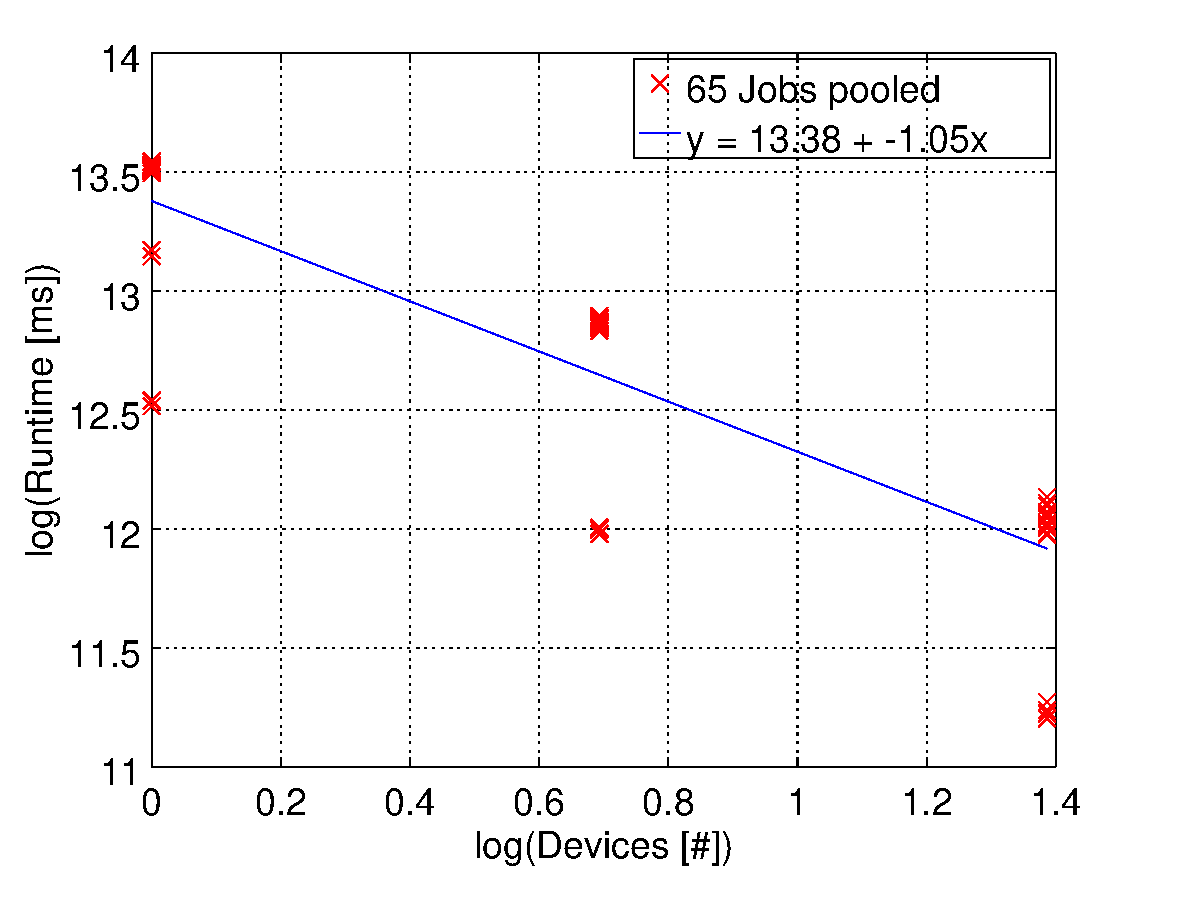
\includegraphics[width=\textwidth]{runtime-log-workerBacc0}
    \caption{Experiment \ref{M2} Gesamtlaufzeiten mit 1, 2, und 4 Workern, und je 25 Iterationen. X und Y Achse logaritmiert.}
    \label{runtime-log-workerBacc0}
  \end{minipage}
\end{figure}






\clearpage
\section{Empty Jobs - Pool Workflow}
\label{M3}

\begin{wrapfigure}{r}{0.45\textwidth}
  \vspace{-30pt}
  \begin{center}
    \includegraphics{hist-workerBacc1}
    \caption{Experiment \ref{M3} WorkerJob Laufzeiten aller 25 Iterationen in 50bins.}
    \label{hist-workerBacc1}
  \end{center}
\end{wrapfigure}

Dieses Experiment soll den durch die Middleware verursachten Overhead bei Verwendung eines Pool Workflows zeigen. Die im Pool gestarteten WorkerJobs führen keinen Nutz-Algorithmus aus, sie terminieren unmittelbar nach dem Start.
Wie alle anderen Experimente wird auch dieses mit einem, zwei und vier Rechnern mit je vier Workern ausgeführt. Es zeigt sich, dass der Server bereits mit acht Workern, überlastet ist.

Zu erkennen ist dies am Histogramm in Abbildung \ref{hist-workerBacc1}.
Die Laufzeit von RemoteJobs wird am auftraggebenenden Gerät gemessen, inklusive Roundtrip, Serialisierung, und Workflow Logic.
Das Histogramm zeigt schon bei acht, und vor allem bei 16 Workern viel längere Laufzeiten.
Da die tatsächliche Laufzeit am Worker nahezu null ist und angenommen werden kann, dass die Roundtrip Zeit sich nicht wesentlich veränert hat, muss die zusätzliche Laufzeit dem Server zugeschrieben werden.

Erhält der Server von zu vielen Workern Return Messages, wächst die Queue am Server.
Die Auslastung des Servers ist von der Anzahl der Worker, die mit ihm verbunden sind, linear abhängig. Ein HCSNO mit mehreren Worker Ebenen könnte dieses Problem beheben, da es die Serverauslastung logarithmisch von der Gesamtanzahl der Worker abhängig macht. Ein solches System könnte in einer zukünftgien Arbeit untersucht werden.

\vspace{45mm}

\begin{figure}[H]
  \centering
  \begin{minipage}[b]{0.45\textwidth}
    \includegraphics[width=\textwidth]{runtime-box-workerBacc1}
    \caption{Experiment \ref{M3}. Boxplots für Gesamtlaufzeit mit 1, 2, und 4 Worker, und je 25 Iterationen}
    \label{runtime-box-workerBacc1}
  \end{minipage}
  \hfill
  \begin{minipage}[b]{0.45\textwidth}
    \includegraphics[width=\textwidth]{runtime-log-workerBacc1}
    \caption{Experiment \ref{M3} Gesamtlaufzeiten mit 1, 2, und 4 Workern, und je 25 Iterationen. X und Y Achse logaritmiert.}
    \label{runtime-log-workerBacc1}
  \end{minipage}
\end{figure}
